
\chapter{Resultados de la caracterización de los métodos de conexíon en simulación} % Título del Anexo

\label{Resultados-Sim-caract} 

\begin{figure}[H]
    \centering
    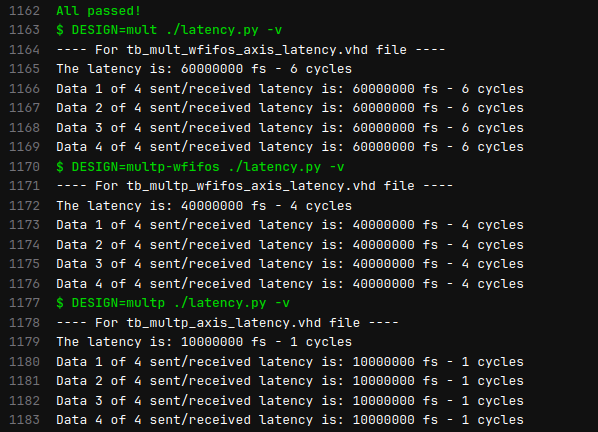
\includegraphics[width=14cm]{Figuras/result/lat1.png}
    \caption{Resultados del ensayo de latencia para Mult-B, Mult-BP y Mult-UBP acoplados mediante \textit{AXI-Stream Verification Componets}.}
    \label{fig:lat1}
\end{figure}

\begin{figure}[H]
    \centering
    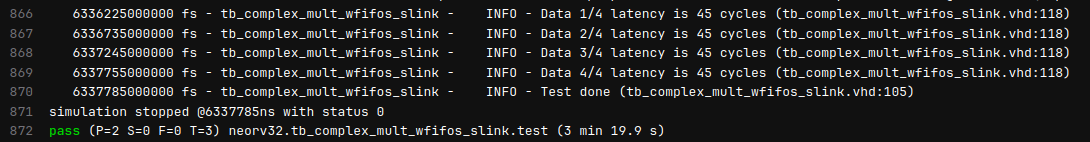
\includegraphics[width=14cm]{Figuras/result/lat2.png}
    \caption{Resultados del ensayo de latencia para NEORV32 + Mult-B, acoplado mediante SLINK.}
    \label{fig:lat2}
\end{figure}

\begin{figure}[H]
    \centering
    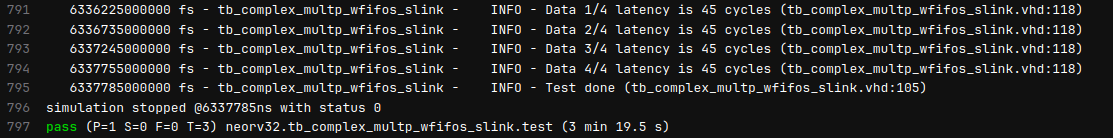
\includegraphics[width=14cm]{Figuras/result/lat3.png}
    \caption{Resultados del ensayo de latencia para NEORV32 + Mult-BP, acoplado mediante SLINK.}
    \label{fig:lat3}
\end{figure}

\begin{figure}[H]
    \centering
    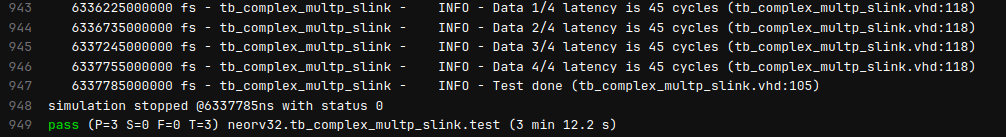
\includegraphics[width=14cm]{Figuras/result/lat4.png}
    \caption{Resultados del ensayo de latencia para NEORV32 + Mult-UBP, acoplado mediante SLINK.}
    \label{fig:lat4}
\end{figure}

\begin{figure}[H]
    \centering
    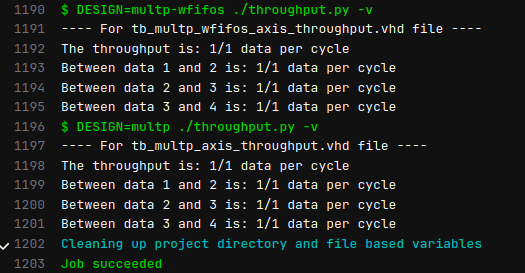
\includegraphics[width=14cm]{Figuras/result/thr1.png}
    \caption{Resultados del ensayo de \textit{throughput} para Mult-B, Mult-BP acoplados mediante \textit{AXI-Stream Verification Componets}.}
    \label{fig:thr1}
\end{figure}

\begin{figure}[H]
    \centering
    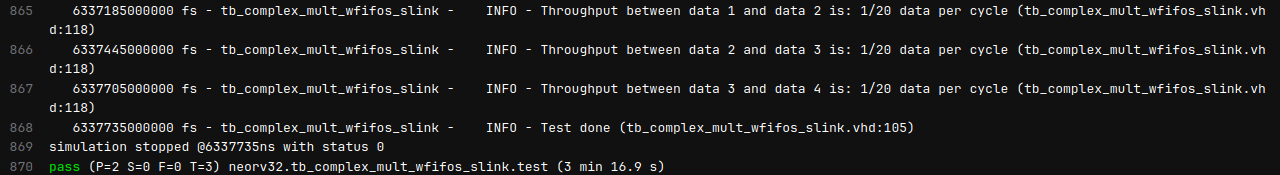
\includegraphics[width=14cm]{Figuras/result/thr2.png}
    \caption{Resultados del ensayo de \textit{throughput} para NEORV32 + Mult-B, acoplado mediante SLINK.}
    \label{fig:thr2}
\end{figure}

\begin{figure}[H]
    \centering
    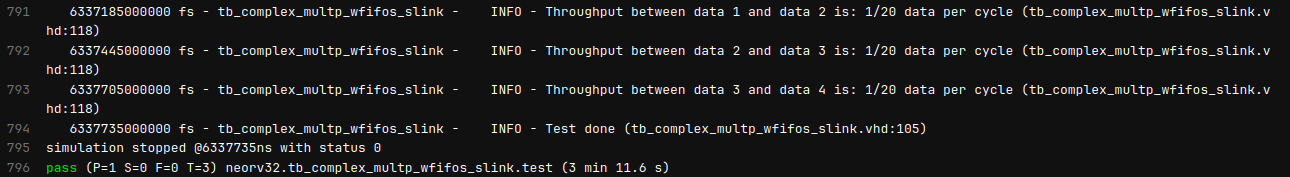
\includegraphics[width=14cm]{Figuras/result/thr3.png}
    \caption{Resultados del ensayo de \textit{throughput} para NEORV32 + Mult-BP, acoplado mediante SLINK.}
    \label{fig:thr3}
\end{figure}

\begin{figure}[H]
    \centering
    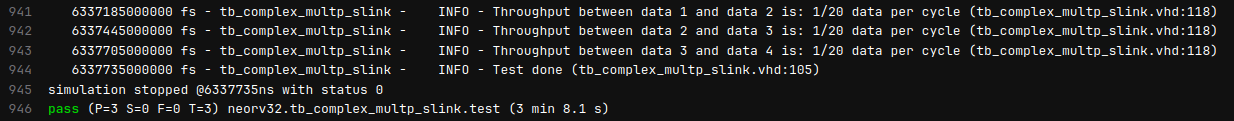
\includegraphics[width=14cm]{Figuras/result/thr4.png}
    \caption{Resultados del ensayo de \textit{throughput} para NEORV32 + Mult-UBP, acoplado mediante SLINK.}
    \label{fig:thr4}
\end{figure}

\begin{figure}[H]
    \centering
    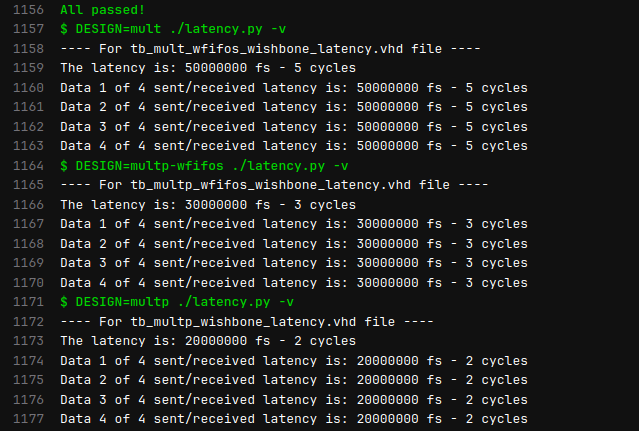
\includegraphics[width=14cm]{Figuras/result/lat5.png}
    \caption{Resultados del ensayo de latencia para Mult-B, Mult-BP y Mult-UBP acoplados mediante \textit{Wishbone Verification Componets}.}
    \label{fig:lat5}
\end{figure}

\begin{figure}[H]
    \centering
    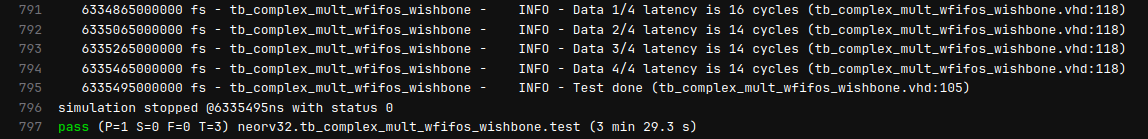
\includegraphics[width=14cm]{Figuras/result/lat6.png}
    \caption{Resultados del ensayo de latencia para NEORV32 + Mult-B, acoplado mediante XBUS.}
    \label{fig:lat6}
\end{figure}

\begin{figure}[H]
    \centering
    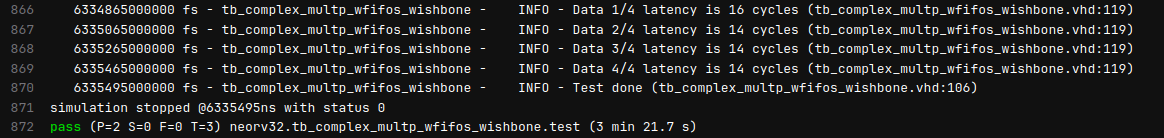
\includegraphics[width=14cm]{Figuras/result/lat7.png}
    \caption{Resultados del ensayo de latencia para NEORV32 + Mult-BP, acoplado mediante XBUS.}
    \label{fig:lat7}
\end{figure}

\begin{figure}[H]
    \centering
    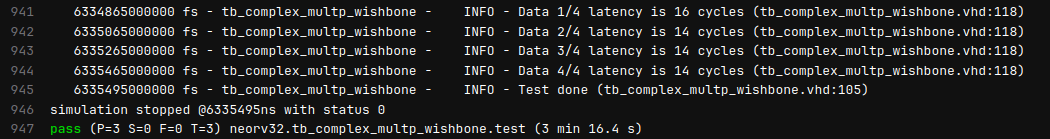
\includegraphics[width=14cm]{Figuras/result/lat8.png}
    \caption{Resultados del ensayo de latencia para NEORV32 + Mult-UBP, acoplado mediante XBUS.}
    \label{fig:lat8}
\end{figure}

\begin{figure}[H]
    \centering
    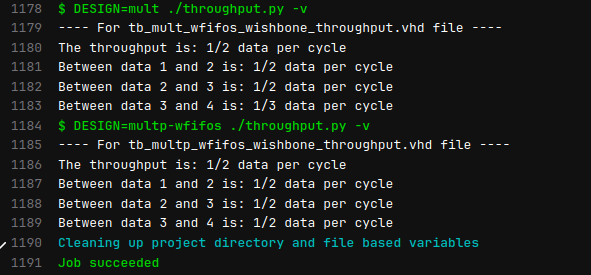
\includegraphics[width=14cm]{Figuras/result/thr5.png}
    \caption{Resultados del ensayo de \textit{throughput} para Mult-B, Mult-BP acoplados mediante \textit{Wishbone Verification Componets}.}
    \label{fig:thr5}
\end{figure}

\begin{figure}[H]
    \centering
    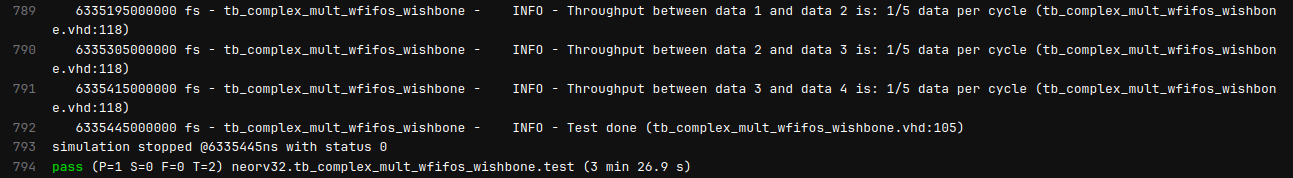
\includegraphics[width=14cm]{Figuras/result/thr6.png}
    \caption{Resultados del ensayo de \textit{throughput} para NEORV32 + Mult-B, acoplado mediante XBUS.}
    \label{fig:thr6}
\end{figure}

\begin{figure}[H]
    \centering
    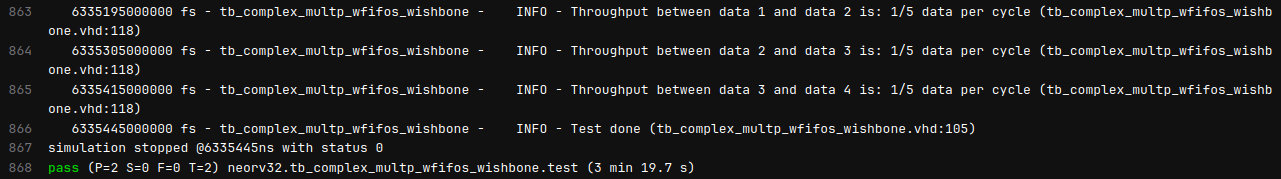
\includegraphics[width=14cm]{Figuras/result/thr7.png}
    \caption{Resultados del ensayo de \textit{throughput} para NEORV32 + Mult-BP, acoplado mediante XBUS.}
    \label{fig:thr7}
\end{figure}

\begin{figure}[H]
    \centering
    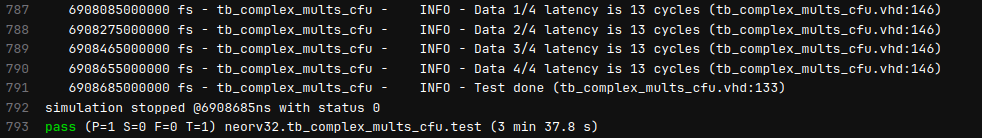
\includegraphics[width=14cm]{Figuras/result/lat9.png}
    \caption{Resultados del ensayo de latencia para NEORV32 + Mult-B, acoplado mediante CFU.}
    \label{fig:lat9}
\end{figure}

\begin{figure}[H]
    \centering
    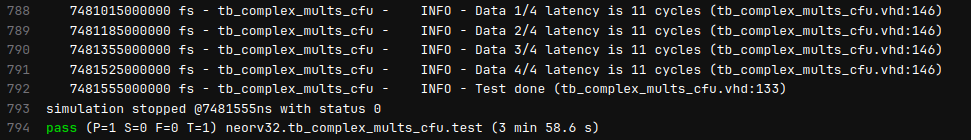
\includegraphics[width=14cm]{Figuras/result/lat10.png}
    \caption{Resultados del ensayo de latencia para NEORV32 + Mult-BP, acoplado mediante CFU.}
    \label{fig:lat10}
\end{figure}

\begin{figure}[H]
    \centering
    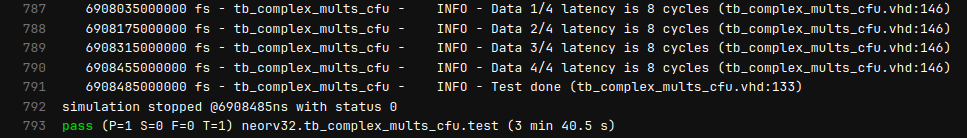
\includegraphics[width=14cm]{Figuras/result/lat11.png}
    \caption{Resultados del ensayo de latencia para NEORV32 + Mult-UBP, acoplado mediante CFU.}
    \label{fig:lat11}
\end{figure}

\begin{figure}[H]
    \centering
    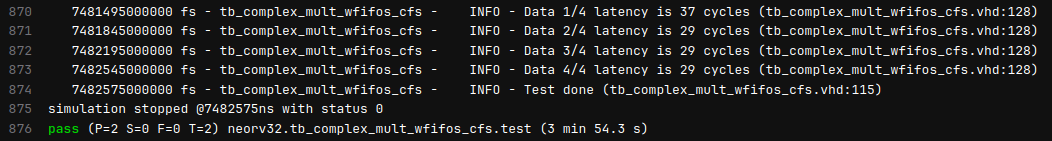
\includegraphics[width=14cm]{Figuras/result/lat12.png}
    \caption{Resultados del ensayo de latencia para NEORV32 + Mult-B, acoplado mediante CFS.}
    \label{fig:lat12}
\end{figure}

\begin{figure}[H]
    \centering
    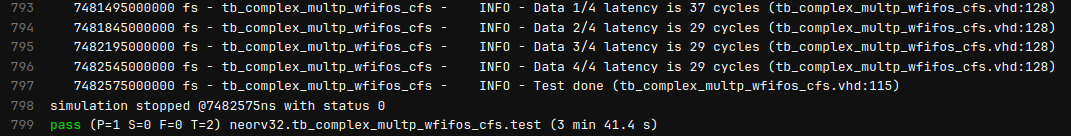
\includegraphics[width=14cm]{Figuras/result/lat13.png}
    \caption{Resultados del ensayo de latencia para NEORV32 + Mult-BP, acoplado mediante CFS.}
    \label{fig:lat13}
\end{figure}

\begin{figure}[H]
    \centering
    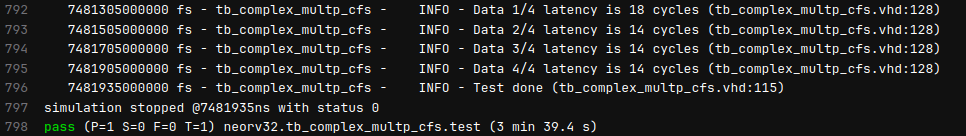
\includegraphics[width=14cm]{Figuras/result/lat14.png}
    \caption{Resultados del ensayo de latencia para NEORV32 + Mult-UBP, acoplado mediante CFS.}
    \label{fig:lat14}
\end{figure}

\begin{figure}[H]
    \centering
    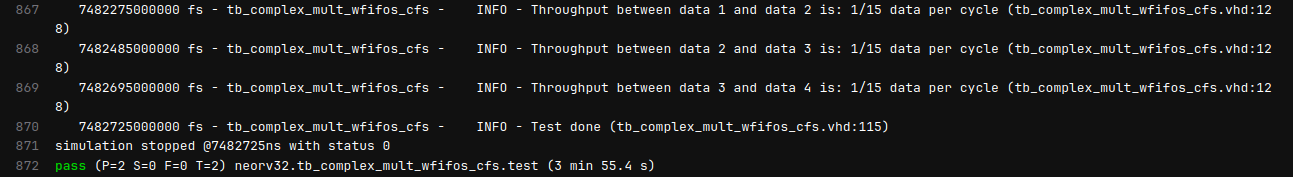
\includegraphics[width=14cm]{Figuras/result/thr8.png}
    \caption{Resultados del ensayo de \textit{throughput} para NEORV32 + Mult-B, acoplado mediante CFS.}
    \label{fig:thr8}
\end{figure}

\begin{figure}[H]
    \centering
    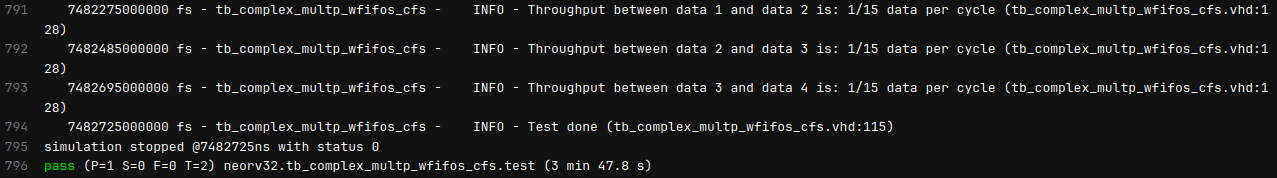
\includegraphics[width=14cm]{Figuras/result/thr9.png}
    \caption{Resultados del ensayo de \textit{throughput} para NEORV32 + Mult-BP, acoplado mediante CFS.}
    \label{fig:thr9}
\end{figure}
